\documentclass{article}
\usepackage{graphicx}
\usepackage[affil-it]{authblk}
\usepackage{url}
\usepackage{nth}
\usepackage{float}
\usepackage{multirow}
\usepackage{hyperref}
\usepackage{subfig}

\begin{document}

\title{Developing a driver for a film scanner by means of USB sniffing and reverse engineering}
\author{Hugo Platzer \\ University of Salzburg}
\maketitle

\section{Introduction}

Describe the scanner and motivation

\section{The USB standard}

\subsection{Motivation}

USB is an interface intended to connect various peripherals to PCs. These include:
Human interface devices like keyboards and mice; storage devices like card readers,
external hard disks, memory sticks and smartphones; multimedia devices like microphones, speakers,
cameras and scanners. Some highlights leading to its wide adoption \cite[p. 11]{usbstd}:

\begin{itemize}
  \item Unified interface for all kinds of peripherals
  \item Plug and play: The user plugs in the device, the configuration (e.g. loading the appropriate drivers)
  is done automatically by the operating system
  \item Number of ports can be increased using hubs. Multiple hubs can be chained
        allowing for up to 127 devices on a single root port.
  \item High data rate of 480 Mbit / s (USB 2.0 high-speed mode). Also offers low-latency
        transfers for real-time audio/video applications
  \item Backwards compatibility: Older USB 1.1 devices can be used at 2.0 hosts.
        High-speed USB 2.0 devices can also be used on older
        machines supporting only USB 1.1 (albeit at lower speed).
\end{itemize}

\subsection{Electrical side}

\begin{figure}[!htbp]
  \caption{USB cable cross-section \cite[p. 17]{usbstd}}
  \centering
  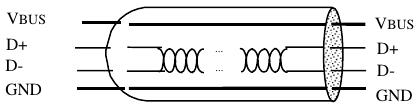
\includegraphics[width=0.5\textwidth]{images/usb_cable.jpg}
\end{figure}

A USB cable has four wires: One as ground, VBUS for a 5 V power supply and two for data transmission.
The power line allows it to draw up to 100 mA without any configuration. This is useful for simple
devices that are not using the data lanes, just the power, like USB lights. Also it allows for devices
not taking much power to be self-powered which eliminates the need for an extra power supply and connector.
Devices can ask the host for more power (up to 500 mA), those that need even more (like a lot of scanners) need
an external supply. \cite[p. 17f.]{usbstd}

\subsection{Signaling}

\subsubsection{Low-level states}

USB is a serial bus which means there is only a single path for data transmission.
Differential signalling across the D- and D+ wires is used, which means the difference in voltage
across the two wires (rather than some absolute) determines the state. This is beneficial because
noise during transmission should affect both lines equally, not changing the difference.
Higher frequencies and thus data rates become possible.

\begin{table}[!htbp]
  \caption{USB speed modes \cite[p. 159]{usbstd}}
  \centering
  \begin{tabular}{l | l | l}
    Mode & Speed & Bit time \\ \hline
    Low Speed & 1.5 Mbit / s & 667 ns \\
    Full Speed & 12 Mbit / s & 83 ns \\
    High Speed & 480 Mbit / s & 2 ns \\
  \end{tabular}
\end{table}

\begin{table}[!htbp]
  \caption{Low-level data line states (only applies to Full Speed) \cite[p. 145]{usbstd}}
  \centering
  \begin{tabular}{l | l}
    Levels & State \\ \hline
    Differential '0' & D- high, D+ low \\
    Differential '1' & D- low, D+ high \\
    Single Ended Zero (SE0) & both low \\
    Single Ended One (SE1) & both high (illegal state, should never happen) \\
    Data 'J' state & Differential '1' \\
    Data 'K' state & Differential '0' \\
    Idle state & Data 'J' state \\
    Start of Packet (SOP) & Switch from idle to 'K' \\
    End of Packet (EOP) & SE0 for 2 bit times followed by 'J' for 1 bit time \\
    Disconnect & SE0 for $\geq$ 2 us \\
    Connect & Idle for 2.5 us \\
    Reset & SE0 for $\geq$ 2.5 us \\
  \end{tabular}
\end{table}

\pagebreak
Low Speed is used for devices where speed is not important (mice, keyboards).
It allows for cheaper cables and electronics. High Speed is only available
in USB 2.0. For reasons of simplicity, only full speed signaling will be covered
here. \cite[p. 12]{usbstd}

SE0 is the state of the data lines if no device is connected. The host
recognizes a device being plugged in by the D+ line being "pulled up" to high.
It then most likely initiates a reset so the device is in a known state for
communication to begin. Similarly, a disconnect is sensed by a SE0 for some time.
\cite[p. 149]{usbstd}

It is important to note that {\bf all communication on the USB bus is initiated by the
host}. Devices on the bus can not directly talk to each other and can only talk
to the host as a direct response to a request made by it before.
\cite[p. 27]{usbstd}

\subsubsection{Bitstream encoding}

USB uses NRZI encoding for the transmitted data: A zero is represented by a change to
the opposite state while a one is represented by staying in the same state.

\begin{figure}[!htbp]
  \caption{NRZI bitstream encoding \cite[p. 157]{usbstd}}
  \centering
  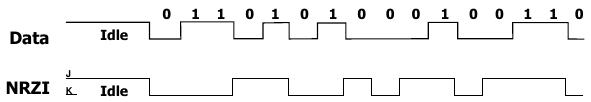
\includegraphics[width=0.5\textwidth]{images/nrzi_encoding.jpg}
\end{figure}

For keeping the receiver clock in sync with the data it is not ideal if the signal
stays at J or K for too long. To prevent this, a technique called "bit stuffing"
is used: Before doing NRZI encoding, a zero is inserted after every six consecutive ones
in the data. The receiver recognizes the stuffed bits during decoding and discards them.
\cite[p. 157]{usbstd}

\subsection {Packets}

Packets are the atomic unit of data transmission in USB. In between packet transmission,
the bus remains in an idle state. Every packet starts with a sync pattern to synchronize
the clocks between sender and receiver. Next are the actual data bits. The packet is
terminated by an EOP state. Fields in a packet are transmitted least-significant
bit first. \cite[p. 195]{usbstd}

The first 8 bits of every packet contain the packet ID (PID) which identifies its type
and thus how the rest of the packet data should be interpreted. The PID is 4 bits long, they are transmitted a second time in reverse bit order to allow the receiver to quickly
discard a faulty packet. There are 17 different packet types (PRE and ERR have the same ID,
some are only relevant for High Speed) \cite[p. 195]{usbstd}:

\begin{table}[!htbp]
  \caption{USB packet types; notice how the least-significant two bits identify the packet category \cite[p. 196]{usbstd}}
  \centering
  \begin{tabular}{l | l | l | p{5cm}}
    PID type & PID name & \begin{tabular}{@{}l} PID bits \\ (3..0) \end{tabular} & Description \\ \hline
    \multirow{4}*{Token} & OUT & 0001 & Address + endpoint number for host-to-device transaction \\
                         & IN & 1001 & Address + endpoint number for device-to-host transaction \\
                         & SOF & 0101 & Start-of-frame marker, frame number \\
                         & SETUP & 1101 & Special host-to-device transaction for device configuration \\ \hline
    \multirow{4}*{Data} & DATA0 & 0011 & Data packet \\
                         & DATA1 & 1011 & Data packet \\
                         & DATA2 & 0111 & Data packet (only High Speed) \\
                         & MDATA & 1111 & Data packet (only High Speed) \\ \hline
    \multirow{4}*{Handshake} & ACK & 0010 & Receiver accepts error-free data packet \\
                         & NAK & 1010 & Receiver cannot accept data or transmitter cannot send data \\
                         & STALL & 1110 & Endpoint halted or control pipe request not supported \\
                         & NYET & 0110 & Data packet (only High Speed) \\ \hline
    \multirow{4}*{Special} & PRE & 1100 & Preamble to enable downstream traffic to low-speed devices \\
                         & ERR & 1100 & Split Transaction error handshake \\
                         & SPLIT & 1000 & High speed Split Transaction token (only High Speed) \\
                         & PING & 0100 & High speed control flow probe (only High Speed) \\
                         & Reserved & 0000 & Reserved PID \\
  \end{tabular}
\end{table}

\subsubsection{Token packet}

\begin{figure}[H]
  \caption{Token packet format \cite[p. 199]{usbstd}}
  \centering
  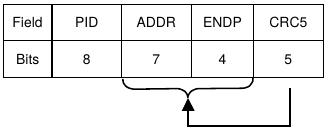
\includegraphics[width=0.5\textwidth]{images/token_packet.jpg}
\end{figure}

Token packets are used at the start of so-called transactions to specify the target
of the transaction on the bus, namely a certain device and endpoint. There are 127
possible devices on a bus (address 0 is reserved for a device that has not been configured yet).
\cite[p. 256]{usbstd}

Endpoints are logical entities on a device that are used as sources and sinks of data
in so-called pipes. A pipe is either in OUT (to device) or IN (to host) direction.
Endpoint 0 is a special bidirectional pipe that must be available on every device
right after the reset. It is used mainly for identifying and configuring the device.
\cite[p. 33]{usbstd}

\subsubsection{Data packet}

\begin{figure}[H]
  \caption{Data packet format \cite[p. 206]{usbstd}}
  \centering
  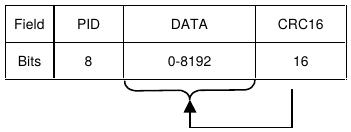
\includegraphics[width=0.5\textwidth]{images/data_packet.jpg}
\end{figure}

Used to transmit the actual data in a transaction.

\subsubsection{Handshake packet}

\begin{figure}[H]
  \caption{Handshake packet format \cite[p. 206]{usbstd}}
  \centering
  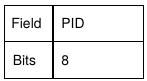
\includegraphics[width=0.21\textwidth]{images/handshake_packet.jpg}
\end{figure}

Used to report the status of a transaction.

\subsection{Transfers}

Transfers are the abstraction level of data exchange as seen at the software
side of the host. From the host's perspective, a transfer transmits a string of
 bytes from / to the device. A transfer is directed to one of the device's endpoints,
each of them has one of four transfer types plus a transfer direction
asscociated with it during device configuration.
Transfers are composed of transactions, which usually consist of three
packets \cite[p. 209ff.]{usbstd}:

\begin{enumerate}
  \item A token packet to tell the type of the transaction and its destination
        (as all USB communication is initiated by the host, the token packet always comes
        from the host)
  \item A DATA packet for the actual payload. Length can vary between 8-64 bytes on Full Speed links.
        This can go host to device or device to host.
  \item A handshake packet (usually ACK, NAK) lets the sender know if the data was received successfully.
\end{enumerate}

Transfers usually consist of multiple transactions.

\begin{figure}[H]
  \caption{Composition of a USB transfer \cite[p. 44]{uc}}
  \centering
  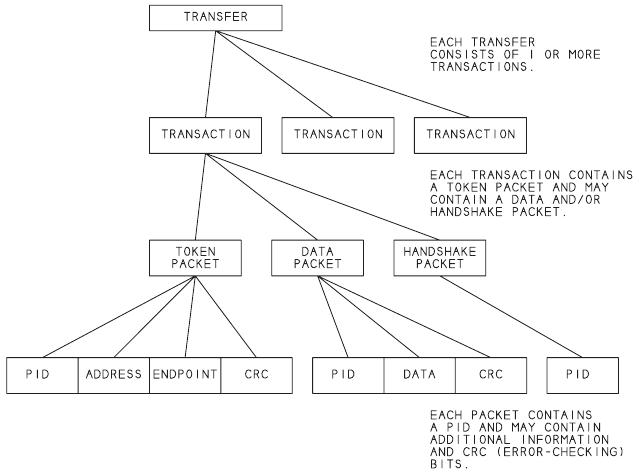
\includegraphics[width=\textwidth]{images/transfer_tree.jpg}
\end{figure}

\subsubsection {Control transfer}

Every device must have endpoint 0 for control transfers. Control endpoints
are message-based. This means each transfer is for a specific message which has
defined length, format and purpose. There can be transfers in either direction
on the same endpoint, although each transfer has a specified (data stage) direction.
Control transfers start with a Setup stage / transaction specifying the target device
and endpoint plus an extra 8 bytes of data called the Device Request. \cite[p. 38f.]{usbstd}

\begin{table}[H]
  \caption{Device Request format \cite[p. 248]{usbstd}}
  \centering
  \begin{tabular}{l | l | l | p{5.5cm}}
    \begin{tabular}{@{}l} Offset \\ (bytes) \end{tabular} & Field &
    \begin{tabular}{@{}l} Size \\ (bytes) \end{tabular} & Description \\ \hline
    
    0 & bmRequestType & 1 &
    
      Bits 0..4: Recipient
      
      \begin{tabular}{l l}
        0 & Device \\
        1 & Interface \\
        2 & Endpoint \\
        3 & Other \\
        4..31 & Reserved \\
      \end{tabular}
      
      \vspace{3mm}
      Bits 5..6: Type
      
      \begin{tabular}{l l}
        0 & Standard \\
        1 & Class \\
        2 & Vendor \\
        3 & Reserved \\
      \end{tabular}
      
      \vspace{3mm}
      Bit 7: Transfer direction
      
      \begin{tabular}{l l}
        0 & Host to device \\
        1 & Device to host \\
      \end{tabular} \\ \hline
  
    1 & bRequest & 1 & Specific request \\ \hline
    2 & wValue & 2 & Varies according to request \\ \hline
    4 & wIndex & 1 & Varies according to request, typically used
    for a index or offset \\ \hline
    6 & wLength & 2 & Number of bytes to be transferred in the data stage
    (0 means no data stage) \\
  \end{tabular}
\end{table}

Depending on the kind of control transfer, there may be a data stage
consisting of data transactions, but this is not required. If there
are data transactions, all are going in the same direction as specified
by the request type.
The transfer is completed with a Status transaction to report back
about the success of the whole transfer.

Control transfers are used right after the device reset to get information about
its capabilities and set a configuration. For this, there are 11 bRequest values
called Standard Requests that have to be supported by all devices as part of the standard.

\begin{table}[H]
  \caption{Some important Standard Requests \cite[p. 250]{usbstd}}
  \centering
  \begin{tabular}{l | l | p{2cm} | p{2cm}}
    bRequest & \begin{tabular}{@{}l}  bmRequestType \\ (7..0) \end{tabular}
     & wValue & wIndex \\ \hline
    
    GET\_DESCRIPTOR & 10000000 & Descriptor type and index & Zero or Language ID \\ \hline
    SET\_ADDRESS & 00000000 & Device address & Zero \\ \hline
    GET\_STATUS & \begin{tabular}{@{}l}  10000000 \\ 10000001 \\ 10000010 \end{tabular}
    & Zero & \begin{tabular}{@{}l}  Zero \\ Interface \\ Endpoint \end{tabular} \\ \hline
    SET\_CONFIGURATION & 00000000 & Configuration value & Zero \\
  \end{tabular}
  
  \vspace{5mm}
  \begin{tabular}{l | l | p{5cm}}
    bRequest & wLength & Data \\ \hline
    
    GET\_DESCRIPTOR & Descriptor length & Descriptor \\
    SET\_ADDRESS & None & None \\
    GET\_STATUS & Two & Device, Interface or endpoint status \\
    SET\_CONFIGURATION & None & None \\
  \end{tabular}
\end{table}

They are also used to control the device after the configuration phase during normal operation.
There are standardized requests (Class Requests) for certain device classes like keyboards, storage devices etc.

Other non-standard devices have custom, vendor-specific requests that are not documented
in the USB standard.

\subsubsection {Bulk transfer}

Bulk transfers are used to transmit large amouts of data with guaranteed delivery
and low overhead but no latency / bandwidth constraints.
Compared to control transfers, they are stream-based. This means there is no defined message
format or size. For an IN endpoint, the host would poll the device endpoint for data until it receives
(cumulative) as many bytes as requested by the software. A transfer can also be ended by the device sending
a data transaction of less size than the maximum of this endpoint (data is always split so there is at most one
smaller packet at the end) or a zero-size data transaction. To avoid data packets being lost, they
alternate between the DATA0 / DATA1 PIDs. A single bulk endpoint is only for incoming
or only for outgoing transfers.
The host schedules them at times when the bus bandwidth is not used by other transfer types.
Typical uses for bulk transfers are transferring data from/to an external harddrive,
to a printer or from a scanner. \cite[p. 52ff.]{usbstd}

\subsubsection {Interrupt transfer}

On the bus, interrupt transfers look the same as bulk transfers.
The main difference is scheduling: The host guarantees that a transfer
attempt is made as often as specified in the endpoint descriptor (1 - 100 ms).
Despite the name, interrupt transfers have nothing to do with hardware interrupts.
All communication on the USB bus is initiated by the host, so it has to poll the device
for data.
Typical uses for interrupt transfers are receiving keypresses from keyboards and
movements from mice. \cite[p. 48ff.]{usbstd}

\subsubsection {Isochronous transfer}

Isochronous transfers are for transmitting data at a constant rate with guaranteed
latency. Compared to interrupt transfers, they offer a guaranteed transfer rate
(with interrupt transfers the interval between two transfers can be anywhere
between zero and the specified maximum). The drawback is a lack of any handshake
/ retry mechanism.
Typical uses for isochronous transfers are USB sound cards or webcams.
\cite[p. 44ff.]{usbstd}

\subsection{Device initialization}
\label{devinit}

The process from a device being plugged in to it becoming usable for the user
roughly goes as follows (every USB bus has at least a root hub device interacting with
the operating system) \cite[p. 87ff.]{uc}:

\begin{enumerate}
  \item The hub detects the device by the change in levels on the data lines.
  \item The hub reports the device to the host.
  \item The host tells the hub to reset the device so communication can begin.
  \item The host assigns an address to the new device.
  \item The host asks for the Device Descriptor to get information identifying the device
        (vendor / product ID, device class).
  \item The host looks for a driver handling this VID / PID combination, if it does not find one,
        it leaves the device in an unconfigured state.
  \item If a driver is found, it is loaded. The device is asked for its configuration profiles.
        The driver sets a configuration and can now make the device serve its purpose.
\end{enumerate}

\subsubsection{Device descriptor}

After setting the address, a GET\_DESCRIPTOR
device request is made, asking for the device descriptor.

\begin{table}[H]
  \caption{Device descriptor format \cite[p. 262f.]{usbstd}}
  \centering
  \begin{tabular}{l | l | l | p{5.5cm}}
    \begin{tabular}{@{}l} Offset \\ (bytes) \end{tabular} & Field &
    \begin{tabular}{@{}l} Size \\ (bytes) \end{tabular} & Description \\ \hline
    
    0 & bLength & 1 & Descriptor size in bytes \\
    1 & bDescriptorType & 1 & 1 for DEVICE descriptor \\
    2 & bcdUSB & 2 & USB specification release number \\
    4 & bDeviceClass & 1 & Class code \\
    5 & bDeviceSubclass & 1 & Subclass code \\
    6 & bDeviceProtocol & 1 & Protocol code \\
    7 & bMaxPacketSize0 & 1 & Maximum packed size for Endpoint 0  \\
    8 & idVendor & 2 & Vendor ID \\
    10 & idProduct & 2 & Product ID \\
    12 & bcdDevice & 2 & Device release number \\
    14 & iManufacturer & 1 & Index of manufacturer string descriptor \\
    15 & iProduct & 1 & Index of product string descriptor \\
    16 & iSerialNumber & 1 & Index of serial number string descriptor \\
    17 & bNumConfigurations & 1 & Number of possible configurations \\
  \end{tabular}
\end{table}


{\bf bDeviceClass} Classes are types of devices that were standardized in USB.
There are class codes for audio devices, human interface devices, storage devices etc.
There is also a vendor-specific class code for devices not conforming to a standardized class.
They are further divided into subclasses specifying the actual functionality more
precisely (i.e. keyboard vs. mouse for HID device).

{\bf idVendor} is a 16-bit identifier assigned by the USB Implementers Forum
for each manufacturer of USB compliant devices. Manufacturers must apply
for a unique ID there.

{\bf idProduct} is a 16-bit identifier assigned by the manufacturer
of the device. Manufacturers manage their own PID space so that IDs
are unique per device.



\subsubsection{Configuration descriptor}

Configurations are profiles that define one or more interfaces for the device
and their characteristics.
Only one configuration can be active at a time.
\cite[p. 244]{usbstd}

\begin{table}[H]
  \caption{Configuration descriptor format \cite[p. 265]{usbstd}}
  \centering
  \begin{tabular}{l | l | l | p{5.5cm}}
    \begin{tabular}{@{}l} Offset \\ (bytes) \end{tabular} & Field &
    \begin{tabular}{@{}l} Size \\ (bytes) \end{tabular} & Description \\ \hline
    
    0 & bLength & 1 & Descriptor size in bytes \\
    1 & bDescriptorType & 1 & 2 for CONFIGURATION descriptor \\
    2 & wTotalLength & 2 & Total length of all descriptors for this configuration \\
    4 & bNumInterfaces & 1 & Number of interfaces in this configuration \\
    5 & bConfigurationValue & 1 & Value to be used to select this configuration with SET\_CONFIGURATION \\
    6 & iConfiguration & 1 & Index of string descriptor for this configuration \\
    7 & bmAttributes & 1 & Bitmap of configuration characteristics (Self-powered etc.) \\
    8 & bMaxPower & 1 & Maximum power consumption from bus in this configuration (mA) \\
  \end{tabular}
\end{table}

\subsubsection{Interface descriptor}

Interfaces are sets of related endpoints that together provide a certain feature
of the device. Deiices can have multiple active interfaces at the same time.
Additionally, interfaces can have alternate settings that change its endpoints' characteristics.
\cite[p. 244]{usbstd}

Device drivers are often assigned to serve a specific interface rather than an entire device.

\begin{table}[H]
  \caption{Interface descriptor format \cite[p. 268f.]{usbstd}}
  \centering
  \begin{tabular}{l | l | l | p{5.5cm}}
    \begin{tabular}{@{}l} Offset \\ (bytes) \end{tabular} & Field &
    \begin{tabular}{@{}l} Size \\ (bytes) \end{tabular} & Description \\ \hline

    0 & bLength & 1 & Descriptor size in bytes \\
    1 & bDescriptorType & 1 & 4 for INTERFACE descriptor \\
    2 & bInterfaceNumber & 1 & Number identifying this interface \\
    3 & bAlternateSetting & 1 & Value specifying alternate setting for this interface \\
    4 & bNumEndpoints & 1 & Number of endpoints in this interface (excluding default endpoint 0) \\
    5 & bInterfaceClass & 1 & Type of functionality provided by interface (similar to Device class) \\
    6 & bInterfaceSubClass & 1 & Subclass of device type (similar to Device class) \\
    7 & bInterfaceProtocol & 1 & Protocol of class-specific requests made for this interface \\
    8 & iInterface & 1 & Index of string descriptor for this interface \\
  \end{tabular}
\end{table}

\subsubsection{Endpoint descriptor}

Endpoint descriptors specify an endpoint's address, type and polling interval.

\begin{table}[H]
  \caption{String descriptor format \cite[p. 269ff.]{usbstd}}
  \centering
  \begin{tabular}{l | l | l | p{5.5cm}}
    \begin{tabular}{@{}l} Offset \\ (bytes) \end{tabular} & Field &
    \begin{tabular}{@{}l} Size \\ (bytes) \end{tabular} & Description \\ \hline
    0 & bLength & 1 & Descriptor size in bytes \\
    1 & bDescriptorType & 1 & 5 for ENDPOINT descriptor \\
    2 & bEndpointAddress & 1 & Bits 3..0 give endpoint number, bit 7 gives endpoint direction
        (0 - out, 1 - in) \\
    3 & bmAttributes & 1 & Bits 1..0 describe endpoint type (Control, Isochronous, Bulk, Interrupt).
        Bits 5..2 specify extra options for isochronous endpoints \\
    4 & wMaxPacketSize & 2 & maximum packet size of the endpoint \\
    6 & bInterval & 1 & How often the host should poll for data (in microframes)
  \end{tabular}
\end{table}

\subsubsection{String descriptor}

String descriptors provide information about the device in human-readable form.
String descriptor 0 transmits language codes supported by the device.

\begin{table}[H]
  \caption{String descriptor format \cite[p. 273f.]{usbstd}}
  \centering
  \begin{tabular}{l | l | l | p{5.5cm}}
    \begin{tabular}{@{}l} Offset \\ (bytes) \end{tabular} & Field &
    \begin{tabular}{@{}l} Size \\ (bytes) \end{tabular} & Description \\ \hline
    0 & bLength & 1 & Descriptor size in bytes \\
    1 & bDescriptorType & 1 & for STRING descriptor \\
    2 & bString & rest & String, UNICODE encoded
  \end{tabular}
\end{table}

\section{USB sniffing}

USB sniffing is the process of recording communication on the USB bus.
This is useful for device developers, driver developers, keyloggers etc.

\subsection{Hardware vs. software sniffing}

Hardware sniffing uses a dedicated device that sits on the bus in between the
host and device. Dedicated software is used to interpret the low-level signals
as packets / transactions.

Software sniffing does not use dedicated hardware to listen to the signals
on the wires. Instead, the host operating system reports packets sent / received
to some software running on the same host.

\paragraph*{Advantages of hardware USB analyzers \cite{analyzerbenefits}}:

\begin{itemize}
\item Independent of the host, not affected by bugs in its USB hardware / software
\item Allow analysis down to the lowest level (voltage levels between wires)
\item See all packets transmitted, including unsuccessful transactions etc.
\end{itemize}

\paragraph*{Advantages of purely software USB analyzers:}

\begin{itemize}
\item Lower cost (free when using usbmon / Wireshark)
\item Easy setup, convenient, no extra hardware required
\end{itemize}

\subsection{usbmon}

{\it usbmon} is a module for the Linux kernel that allows access to
USB request blocks (URBs) as they are being processed. URBs are a
data structure of the Linux kernel and loosely correspond to USB transfers. \cite{usbmon}

\subsubsection{Payload size limitation}

An interesting pitfall when using {\it usbmon} is that for URBs with a payload
longer than 61440 bytes only the first 61440 are captured, the rest is truncated.
Others have faced this problem, unsure where it comes from and what to do: \cite{usbmon_others}

\begin{figure}[H]
  \caption{A large bulk transfer in Wireshark, {\it Data length} $<$ {\it URB length}
           indicates missing bytes.}
  \centering
  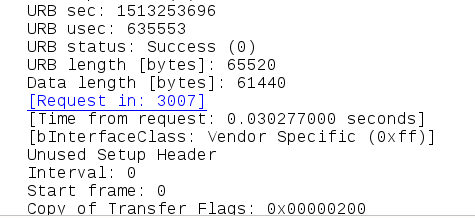
\includegraphics[width=0.8\textwidth]{images/usbmon_missing.png}
\end{figure}

\begin{figure}[H]
  \caption{Image reconstructed from payloads. The frequent tearing is caused by the large
  65520 byte transfers being truncated to 61440 bytes.}
  \centering
  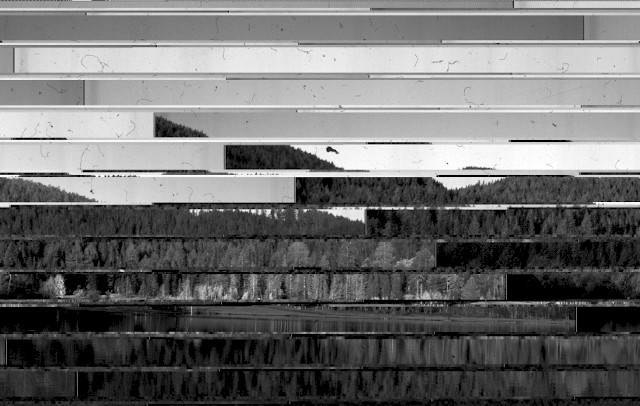
\includegraphics[width=\textwidth]{images/reconstruct_missing.jpg}
\end{figure}

\subsubsection{Kernel patching}
\label{kernelpatch}

Since the problem persisted when changing computers, sniffing software and target devices
it was concluded it must be in the {\it usbmon} kernel module itself.
The {\it linux-source} package (kernel version 4.13) was installed on the {\it Debian 9} system.

Source code for {\it usbmon} is found in {\it drivers/usb/mon}. {\it usbmon} has a
text-based and a binary interface. The binary interface is used by external sniffing
software like Wireshark. The code for it is in {\it mon\_bin.c}.

The magic limit 61440 was not found in the code. However the {\it mon\_bin\_event} procedure
which is involved in extracting data from a current kernel USB event has an interesting statement: \\
\verb|    if (length >= rp->b_size/5) length = rp->b_size/5; |. \\
The default buffer size (this value lands in \verb|rp->b_size|) is defined as \\
\verb|    #define BUFF_DFL   CHUNK_ALIGN(300*1024) |. \\
This gives a maximum length of $\frac{300*1024}{5} = 61440$. Data payloads less
than one fifth of the buffer size are truncated for unknown reasons.
This line was changed to remove the limitation: \\
\verb|    if (length >= rp->b_size) length = rp->b_size; |. \\
The modified kernel was compiled and installed according to standard Debian procedures \cite{debkernel}.
When running this kernel, the full 65520 bytes of payload could be captured.
No adverse side effects were noticed.

\subsection{Wireshark}

Wireshark \cite{wireshark} is a cross-platform sniffing and packet analysis software that
became famous as an Ethernet (network) traffic sniffer.
It can be used both for recording traffic as well as analyzing it.
For analyzing, it comes with many protocol dissectors that subsequently
decode the layers of the packet giving a readable description of the protocol fields'
values and their meaning.

Also part of Wireshark is the {\it tshark} \cite{wireshark_tshark} utility. It is basically
a command-line version of Wireshark, also accessing
the same configuration files, this means behavior of {\it tshark} can be configured
inside Wireshark, for instance which protocols are enabled. {\it tshark} is ideal for scripts
that need to parse the {\it .pcapng} capture files generated by Wireshark.
Packets can be filtered by field values and only the desired fields printed.

Wireshark version 2.2.6 was used, other versions may be significantly different.

\subsubsection{Steps}
\label{sniffingprocess}

\begin{enumerate}
  \item Find the bus the device is on using the {\it lsusb} command.
        Ideally, make sure there are no other devices
        on this bus (except the root hub). Try to plug it into different ports.
  
  \item Load the {\it usbmon} kernel module. ({\it modprobe usbmon} as root)
  
  \item Launch {\it wireshark} as root.
  
  \item Select the {\it usbmon*} input corresponding to the bus found in Step 1 and press Start.
  
  \item When completed, stop the recording and save to disk.
  \end{enumerate}

\subsubsection{Customize columns}

For USB sniffing, it is useful to have the most important packet fields as columns.
This allows a good insight into the data flow at a certain time when scrolling through the packet list.
Also, packets can be sorted using some column, allowing them to be grouped according to endpoint,
payload length etc. 

To manage columns, go to {\it Edit $\,\to\,$ Preferences $\,\to\,$ Columns}. New columns are best added
by right clicking on the desired field in the analysis window and selecting "Apply as column".

A good selection of columns could be:
Packet number, Time, Source, Destination,
Length, Info, Leftover capture data ({\it usb.capdata}).
For going through long sequences of control transfers, columns for the control transfer parameters
({\it bmRequestType, bRequest, wValue, wIndex, Data fragment}) are helpful.

\subsubsection{Disable non-USB protocols}
\label{nonusb}

For USB sniffing, none of the supplied protocol dissectors except USB are helpful.
Even worse, they can get in the way by seeing the first bytes of the data payload match
some pattern which causes them to be interpreted as some protocol while they are just raw pixel
values. For these packets, the {\it usb.capdata} field becomes unavailable which makes their
payload ignored when parsing the capture file. This leads to missing image bytes, noticeable
as a tear in the image (similar to a truncated payload).

To fix this, go to {Analyze $\,\to\,$ Enabled protocols}, click "Disable all" and
then enable only USB. \cite[Section 10.4]{wireshark_userguide}

\subsection{Example}

\subsubsection{Scenario}

To provide some insight into the sniffing process and how the recorded data can be
interpreted, I chose to record keystrokes from a USB keyboard. Since USB keyboards
are very widespread and follow a standard protocol, the experiment can be repeated
by almost anyone.

A bus with no devices on it (except the mandatory root hub with address 1) is chosen
for sniffing.
Recording is started before the device gets attached.
The keyboard is attached, then the following keys are pressed and
then released (one after another): a, b, a. Recording is then stopped.

For brevity, only a few of the captured packets are discussed here.

\subsubsection{Device configuration}

When the device is connected, a process like in \ref{devinit} starts.
The device is reset, an address issued and descriptors queried. The device
descriptor and the interface / endpoint descriptor are shown here.

\begin{figure}[H]
  \caption{Device descriptor of USB keyboard}
  \centering
  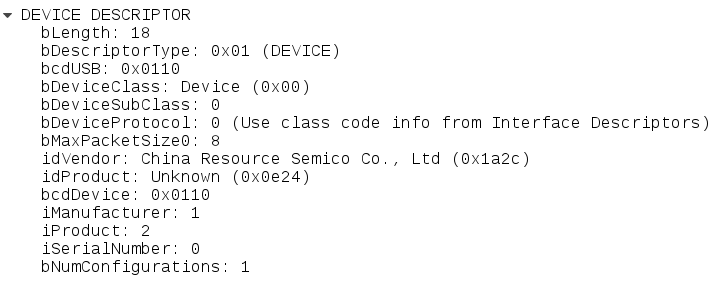
\includegraphics[width=\textwidth]{images/keyboard_sniff1.png}
\end{figure}

The class code of 00 signifies that information about the device should be
obtained from the interface descriptor. The vendor name is queried
from a database by Wireshark (only the 2 byte ID is transmitted over the bus).

\begin{figure}[H]
  \caption{Interface / endpoint descriptor of USB keyboard}
  \centering
  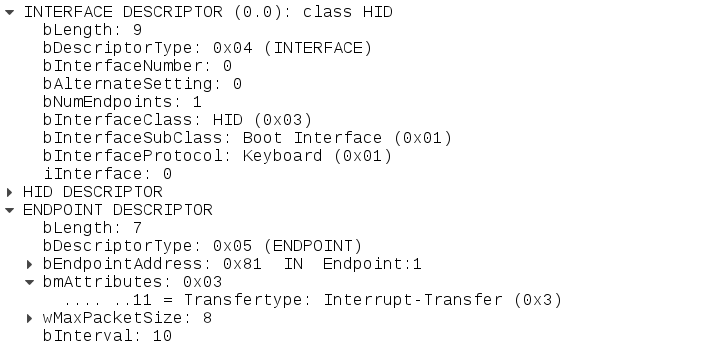
\includegraphics[width=\textwidth]{images/keyboard_sniff2.png}
\end{figure}

The interface identifies as a keyboard and has one extra input endpoint.
Interrupt transfers should be performed there every 10ms.
The data received from the endpoint is an 8-byte HID report giving information
about pressed keys. The first of these bytes describes pressed modifier keys
(Ctrl, Alt etc.) the second byte is reserved, the third byte describes the
actual pressed key. \cite{usbhid}

\subsubsection{Data transmitted while keys are pressed}

\begin{figure}[H]
  \caption{HID reports from USB keyboard}
  \centering
  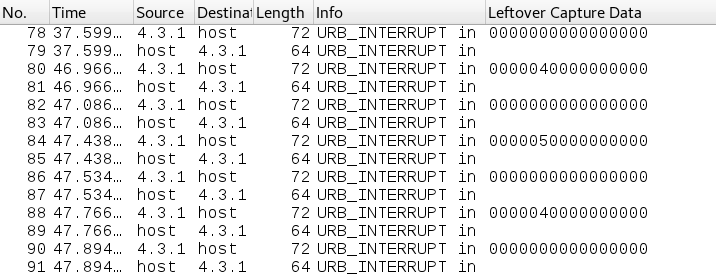
\includegraphics[width=\textwidth]{images/keyboard_sniff3.png}
\end{figure}

In \cite[p.53]{usbusage} the byte values 04 and 05 stand for the a and
b keys respectively.

\subsection{Sniffing using VirtualBox}

When trying to capture device communication from some operating system, it
is convenient to take Linux as a host due to its good sniffing capabilities and
install the target operating system and device driver in a virtual machine.
The virtualization software used here is Oracle VirtualBox \cite{vbox}.

To allow the virtual machine to access the device, the "USB passthrough" feature is used.
This makes the device visible to the guest operating system: VirtualBox
relays communication between the actual device on the host and the virtual device connected
to a virtual USB controller for the guest.
The passthrough is limited to devices with a specified vendor / product ID combination,
new devices can be added by selecting the machine and clicking (Settings $\,\to\,$ USB).

\section{Image extraction}

As a first step, I wanted to reconstruct the transmitted image from the
sniffed communication during a scan. This does not require interaction between
my own software and the scanner, only the capture file is analyzed. Extracting the
image is also a necessary step when implementing actual scanning software.

\subsection{Setup}

The Windows XP operating system was set up inside VirtualBox. The
vendor-supplied CyberView X5 scanner software \cite{cvx5} (version 5.16) was installed.
The scanner was connected to the VM via USB passthrough.

\begin{figure}[H]
  \caption{CyberView X5 software}
  \centering
  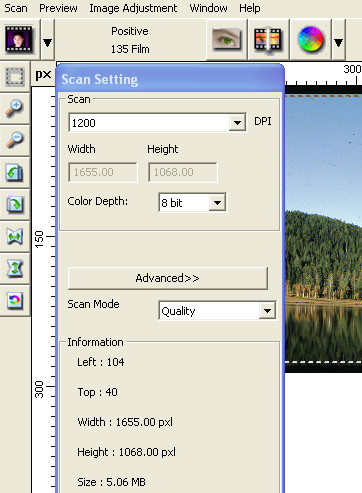
\includegraphics[width=0.75\textwidth]{images/extract_cvx.jpg}
\end{figure}

The scanner software was configured to scan a color positive at default (900 dpi) resolution.
Other settings were left at their default. A prescan (Scan $\,\to\,$ Prescan) was first made to warm up the
scanner lamp so the actual scan (Scan $\,\to\,$ Scan) happens right away. Wireshark recording was started
after completing the prescan, just before starting the actual scan. Recording was stopped
after the scan had completed.

It is important to use a kernel capable of recording the full payload (\ref{kernelpatch})
and also to disable extra protocols in Wireshark (\ref{nonusb}).

A color slide photo of a lake, green / yellow hills, reflections in the water and sky was used as a target.
It allows one to easily know which channel (when having them as separate greyscale images)
is red, green and blue and provides a good impression of overall image quality.

\subsection{Looking at the capture}

\begin{figure}[H]
  \caption{Large bulk transfers}
  \centering
  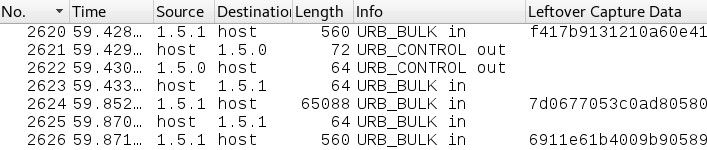
\includegraphics[width=\textwidth]{images/extract_sniff1.jpg}
\end{figure}

The scan took about 20 seconds and generated a capture around 11 megabytes
in size. The image saved by the scanner software was 1655 x 1068 pixels large.
When scrolling through the capture, there are many large bulk transfers
incoming from endpoint 1. It seems likely these contain the image data.
Since scanners work on a line-by-line basis, the pixels are probably
transferred one line after the other.

\begin{figure}[H]
  \caption{Even (dark) and odd (light) offset bytes of payload}
  \centering
  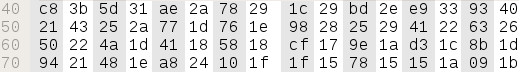
\includegraphics[width=\textwidth]{images/extract_sniff2.jpg}
\end{figure}

When looking at the payload of one of the transfers, bytes with odd offset
have little variation among their neighbors while those with even offset
seem almost random. This suggests the scanner delivers uncompressed
16 bit per pixel little-endian data:
The odd bytes contain the approximate brightness and
the even bytes the fine nuances (noise).

\subsection{Extraction tool}

Since we are likely dealing with uncompressed line-by-line image data,
it should be possible to construct the image by concatenating the payload bytes
and partitioning them into rows. For this, a Python script {\it extractImage.py} was created,
it performs the following steps:

\begin{enumerate}
  \item Load the {\it .pcapng} file generated by Wireshark using {\it tshark} (option {\it --inputFile}).
        Make {\it tshark} print the payload field ({\it usb.capdata}) as hexadecimal for all
        packets on endpoint 1. Parse and concatenate the lines of {\it tshark}'s output into
        one string of bytes.
  
  \item Apply an offset to the bytes and only keep every n-th (options {\it --byteOffset}, {\it --byteNth}).
        This removes unwanted data at the beginning and only keeps the high byte of the 2 bytes per pixel.
  
  \item Break up the byte string into same-size chunks of a specified size (option {\it --lineLength}),
        each representing a line of the image.

  \item Apply an offset to the lines and only keep every n-th (options {\it --lineOffset}, {\it --lineNth}).
  
  \item Drop all lines beyond a specified maximum (option {\it --lineMax}). This removes abnormal lines at the
        end and brings all color channels to the same dimensions.

  \item Create a grayscale PNG image, dimensions are the line width and the number of remaining lines.
        Write the PNG file (option {\it --outputFile}).
\end{enumerate}

\subsection{Results}

\subsubsection{First attempts}

\begin{figure}[H]
    \centering
    \subfloat[width 1655]{{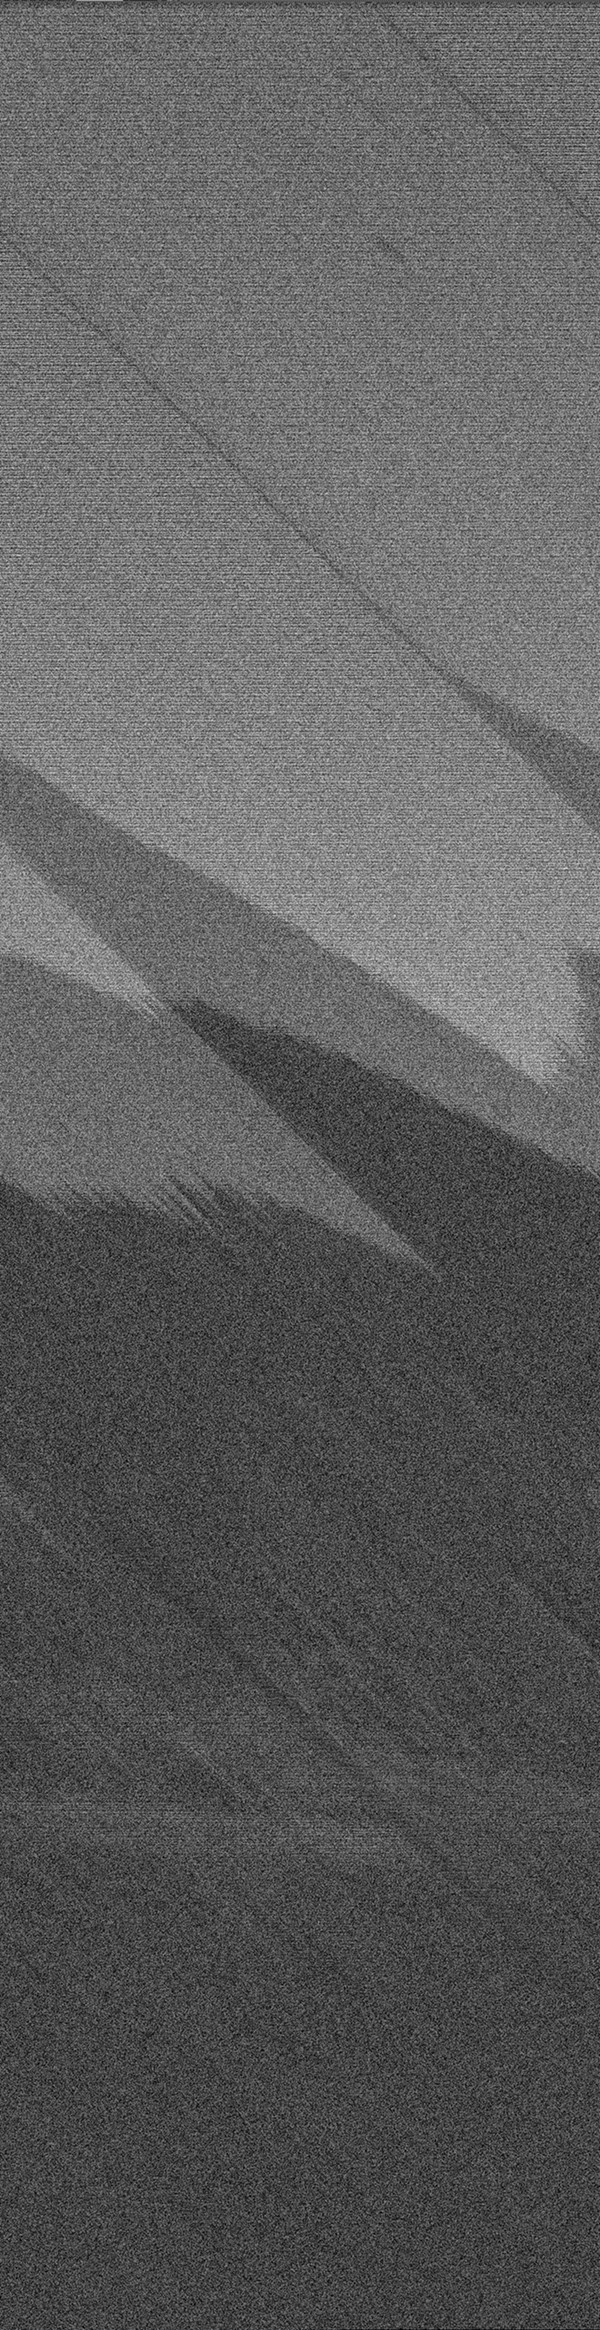
\includegraphics[width=2cm]{images/extract_result1.jpg} }}
    \qquad
    \subfloat[every 2nd byte, width 1655]{{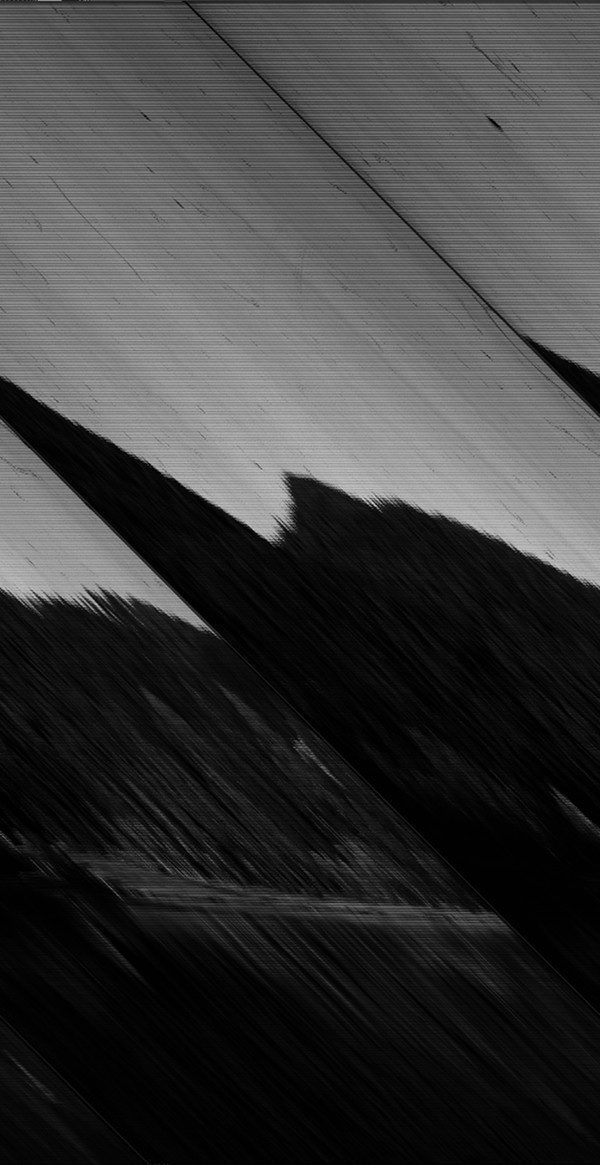
\includegraphics[width=4cm]{images/extract_result2.jpg} }}
    \qquad
    \subfloat[every 2nd byte, width 1653]{{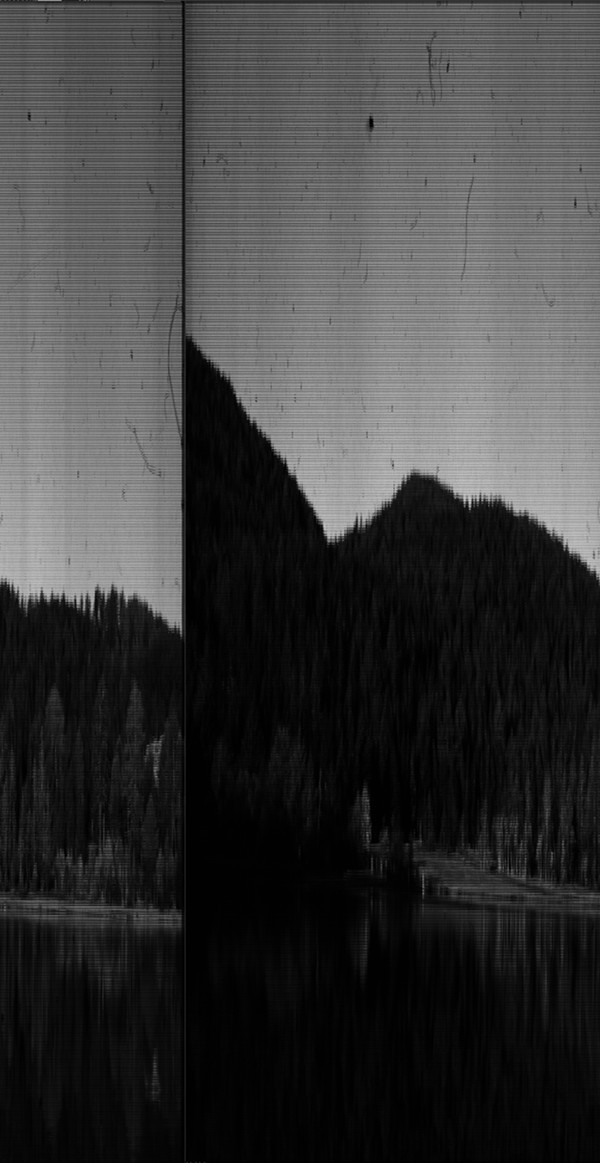
\includegraphics[width=4cm]{images/extract_result3.jpg} }}
    \caption{First attempts at image extraction}
    \label{extraction_first}

\end{figure}

As a first guess, the line width was set to the line width of the saved image (1653 px).
This produced the result in \autoref{extraction_first} a). It clearly resembles some image but there
is work to be done. Since there are two bytes per pixel, I tried keeping only every second byte
starting from the first. This looked like \autoref{extraction_first} b). The noise is now gone which means
I have kept the high bytes. The shapes being distorted points to a slightly off line width.
The correct line width seems to be 1653 as seen in \autoref{extraction_first} c).

\subsubsection{Byte offset}

\begin{figure}[H]
    \centering
    \subfloat[offset 0]{{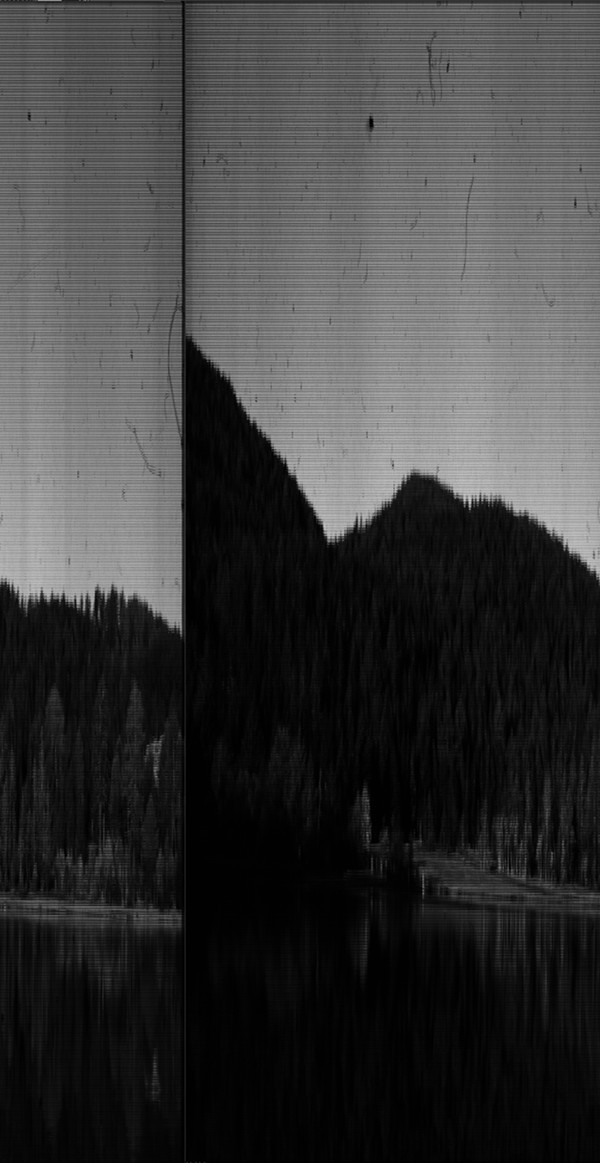
\includegraphics[width=3.5cm]{images/extract_result3.jpg} }}
    \quad
    \subfloat[offset 766]{{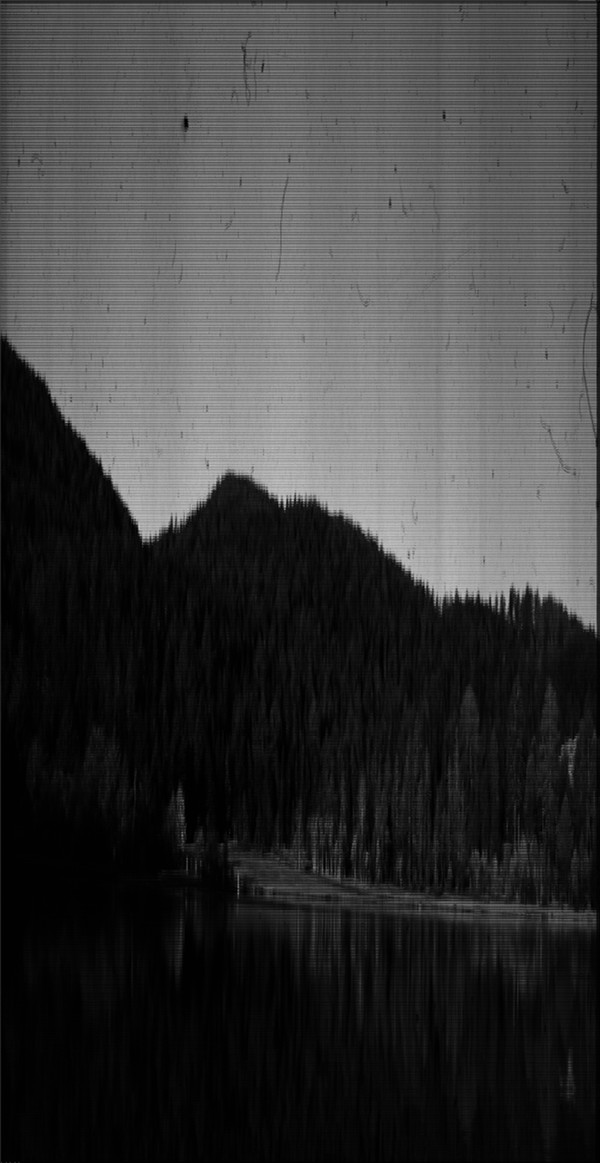
\includegraphics[width=3.5cm]{images/extract_result5.jpg} }}
    \quad
    \subfloat[offset 1300]{{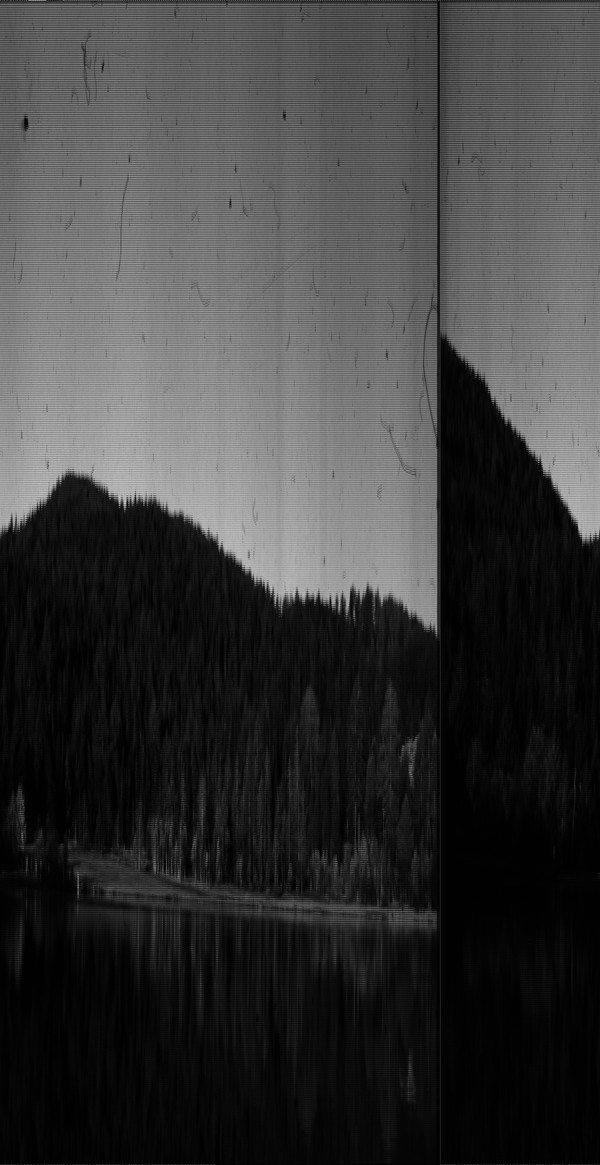
\includegraphics[width=3.5cm]{images/extract_result4.jpg} }}
    \caption{Different byte offsets}
    \label{extraction_offset}

\end{figure}

\subsubsection{Color channel interleaving}

\begin{figure}[H]
    \centering
    \subfloat[every 3rd line, offset 0]{{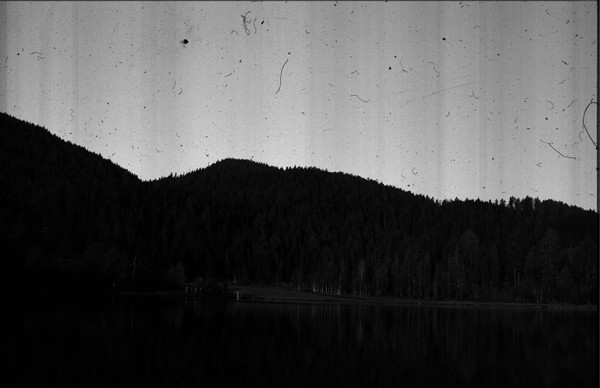
\includegraphics[width=5.5cm]{images/extract_result6.jpg} }}
    \quad
    \subfloat[every 3rd line, offset 1]{{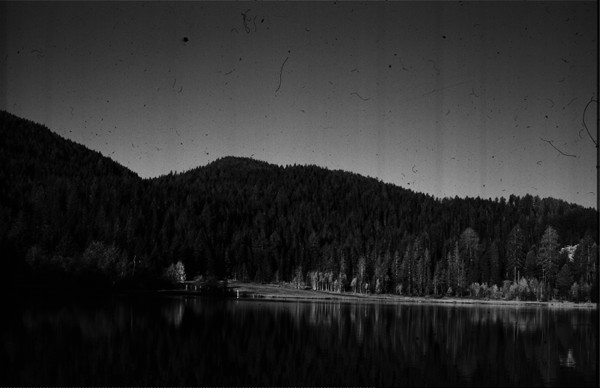
\includegraphics[width=5.5cm]{images/extract_result7.jpg} }}
    \quad
    \subfloat[every 3rd line, offset 2]{{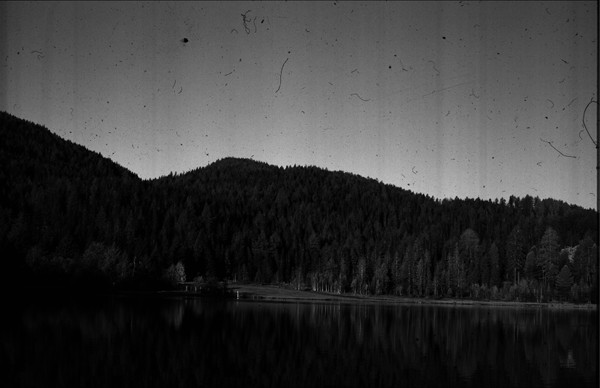
\includegraphics[width=5.5cm]{images/extract_result8.jpg} }}
    \caption{Keeping every 3rd line from various offsets}
    \label{extraction_channel}

\end{figure}

\section{Controlling the device}

\section{Image processing}

\newcounter{firstbib}
\pagebreak

\renewcommand{\refname}{References}
\begin{thebibliography}{}

  \item[]\hspace{-\labelwidth}\hspace{-\labelsep}\textbf{USB standard}

  \bibitem{uc} USB Complete: Everything You Need to Develop
               Custom USB Peripherals (\nth{3} edition).
               Jan Axelson, Lakeview Research LLC 2012.
               ISBN: {\tt   978-1-931448-03-1}
               
  \item[]\hspace{-\labelwidth}\hspace{-\labelsep}\textbf{USB sniffing}
  
  \bibitem{usbmon} The usbmon: USB monitoring framework. Pete Zaitcev,
  Proceedings of the Linux Symposium, Volume Two, July 20-23 2005.
  \setcounter{firstbib}{\value{enumiv}}
\end{thebibliography}

\renewcommand{\refname}{Links}
\begin{thebibliography}{}
  \setcounter{enumiv}{\value{firstbib}}
  
  \item[]\hspace{-\labelwidth}\hspace{-\labelsep}\textbf{USB standard}
  
  \bibitem{usbstd} Universal Serial Bus Specification, Revision 2.0.
                   April 27, 2000. Available at
                   \url{http://www.usb.org/developers/docs/usb20_docs/}

  \item[]\hspace{-\labelwidth}\hspace{-\labelsep}\textbf{USB sniffing}


  \bibitem{analyzerbenefits}
  \url{https://www.totalphase.com/solutions/apps/usb-analyzer-benefits/}

  \bibitem{usbmon_others}
  \url{http://permalink.gmane.org/gmane.linux.usb.general/101338}
  Others describing issues with {\it} usbmon truncated payloads
  
  \bibitem{debkernel}
  \url{https://www.debian.org/releases/stretch/amd64/ch08s06.html.en}

  \bibitem{wireshark}
  \url{https://www.wireshark.org/}
  Homepage of the Wireshark network protocol analyzer
  
  \bibitem{wireshark_tshark}
  \url{https://www.wireshark.org/docs/man-pages/tshark.html}
  
  \bibitem{wireshark_userguide}
  \url{https://www.wireshark.org/docs/wsug_html}
  Wireshark User's Guide

  \bibitem{usbhid}
  \url{http://www.usb.org/developers/hidpage/HID1_11.pdf}
  USB HID Device Class Definition. Describes structure of HID reports
  
  \bibitem{usbusage}
  \url{http://www.usb.org/developers/hidpage/Hut1_12v2.pdf}
  USB HID Usage Tables. Describe meaning of bytes in HID reports

  \bibitem{vbox}
  \url{https://www.virtualbox.org/}

  \bibitem{cvx5}
  \url{https://reflecta.de/de/downloads/drivers2/~nm.50~nc.108/Treiber-und-Software.html}
\end{thebibliography}



\end{document}
